\documentclass{beamer}
\usepackage{graphics}
\usepackage{amsmath,accents}
\usepackage{tikz}
\usetheme{Frankfurt}
\title{Presentation}
\date{\today}
\author{Shukla , Mishra and Jain}

\begin{document}
\maketitle

\section{Content}
\begin{frame}{Contents}

\begin{itemize}
\item Introduction 
\item Theory
\item Methodology
\item Analysis of Numerical Results
\item Summary 
\end{itemize}

\end{frame}

\section{Introduction}
\begin{frame}{Introduction}
   Likhna hai abhi 
\end{frame}

\section{Theory}
\begin{frame}{Theory}

Finite Difference Methods(FDM) are used for solving differential equations by approximating dervatives at the grid points.
\begin{figure}[h]
\centering

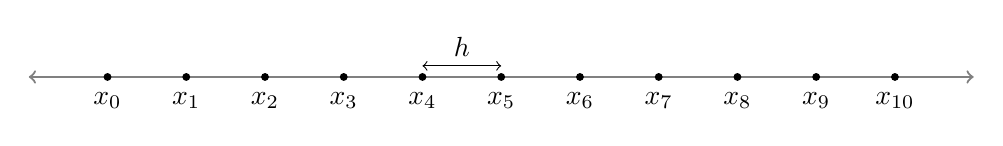
\begin{tikzpicture}
    \coordinate (H) at (4.5,4pt);
    \draw[thick,color=gray,<->] (-1,0) -- (11,0);
    \foreach \x in {0,1,2,3,4,5,6,7,8,9,10}  
        \draw[fill=black] (\x cm,0) circle (1.2pt) (\x cm,-2pt) node[anchor=north] {$x_{\x}$};
    \draw[thin,<->] (4,4pt) -- (5,4pt);%
    \node[anchor=south] at (H) {$h$};
\end{tikzpicture}

\caption{\small 1D mesh with 11 nodes and a meshsize h}
\end{figure}
The difference $h = x_5 - x_4 $ is constant throughout the mesh and $x_4 \equiv x_0 + 4h$.\\

The approximation of first order derivative can be defined as,
{\raggedright 
\begin{align*}
    &\text{} \hspace{1cm} U_x|_i = \lim_{h \to 0} \frac{U_{i+1} - U_i}{h}  \hspace{10mm} \textit{Forward difference} \\
    &\text{or,} \hspace{1cm} U_x|_i = \lim_{h \to 0} \frac{U_{i} - U_{i-1}}{h}  \hspace{9mm} \textit{Backward  difference}\\
    &\text{or,} \hspace{1cm} U_x|_i = \lim_{h \to 0} \frac{U_{i+1} - U_{i-1}}{2h}   \hspace{8mm} \textit{Central difference}
\end{align*}
}
\end{frame}

\begin{frame}
So,in this project we are going to find the electrostatic potential of a capacitor using \textbf{Finite difference Method } and other \textbf{iterative schemes}\footnote{SOR(succesive over relaxation) ,Jacobi, Guass-siedel} and also determining the most appropriate method on the basis of number of iterations. \\

\end{frame}


\end{document}

